\documentclass{article}

\usepackage[a4paper, left=1.5cm, right=1.5cm, top=2cm, bottom=2cm]{geometry}

\usepackage{../../../../components/mathtex}

\usepackage{hyperref}
\usepackage{fancyhdr}
\usepackage{ccicons}
\usepackage{caption}
\usepackage{subcaption}
\usepackage{algorithm}
\usepackage{algorithmic}

% Configuration des en-têtes et pieds de page
\pagestyle{fancy}
\fancyhf{} % reset tout

\fancyhead[L]{DL3 Math-Info AL5}
\fancyhead[C]{Graphes et complexité d'algorithmes}
\fancyhead[R]{2026-2027}

\fancyfoot[L]{Ewen Rodrigues de Oliveira\\\ccbyncsa}
\fancyfoot[R]{\thepage}

\begin{document}

\docTitle{Cours 1 : Définitions de base, représentations des graphes, complexité algorithmique}

\section{Généralités sur les graphes}

\subsection{Définitions et vocabulaire}

\subsection{Graphes}

\definition{
    Un \textbf{graphe} est un couple $G = (V, E)$ où :
    \begin{itemize}
        \item $V$ est un ensemble fini : l'ensemble des \textbf{sommets} de $G$. On le note aussi $V(G)$,
        \item $E$ est un ensemble fini de couples d'éléments de $V$ : l'ensemble des \textbf{arêtes} de $G$. On le note aussi $E(G)$.
    \end{itemize}
}

\remark{De manière intuitive, un graphe est une collection de points (les sommets) reliés par des lignes (les arêtes).}

\example{Un réseau social peut être représenté par un graphe où les sommets représentent les utilisateurs et les arêtes représentent les relations d'amitié entre eux.}

\begin{figure}[h]
    \centering
    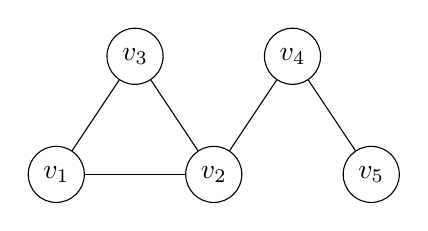
\begin{tikzpicture}
        \node[draw, circle] (v1) at (0, 0) {$v_1$};
        \node[draw, circle] (v2) at (2, 0) {$v_2$};
        \node[draw, circle] (v3) at (1, 1.5) {$v_3$};
        \node[draw, circle] (v4) at (3, 1.5) {$v_4$};
        \node[draw, circle] (v5) at (4, 0) {$v_5$};
        \draw (v1) -- (v2);
        \draw (v2) -- (v3);
        \draw (v3) -- (v1);
        \draw (v2) -- (v4);
        \draw (v4) -- (v5);
    \end{tikzpicture}
    \caption{Exemple d'un graphe simple avec cinq sommets et cinq arêtes.}
\end{figure}

\subsection{Chaînes et chemins}
\subsubsection{Généralités}

\definition{
    Une \textbf{chaîne} dans un graphe $G = (V, E)$ est une suite de sommets de la forme $(v_0, e_1, v_1, e_2, v_2, \ldots, e_n, v_n)$ où :
    \begin{itemize}
        \item $v_i \in V$,
        \item $e_i \in E$,
        \item $e_{i+1} = v_i v_{i+1}$ pour $i = 0, 1, \ldots, n-1$.
    \end{itemize}
}
\vocabulary{Une \textbf{chaîne élémentaire} ou \textbf{chemin} est une chaîne ne passant pas deux fois par un même sommet. Un chemin avec $n$ sommets est noté $P_n$.}

\vocabulary{Une \textbf{chaîne simple} est une chaîne où les arêtes sont deux à deux distinctes \textit{(i.e. qu'on ne repasse pas plusieurs fois par la même arête)}.}


\example{
    \begin{figure}[htbp]
    \centering
    \tikzset{
        vertex/.style={circle, draw, fill=black, inner sep=0pt, minimum size=3pt}
    }

    % Premier graphe : chemin P5
    \begin{subfigure}[t]{0.42\textwidth}
        \centering
        \begin{tikzpicture}[scale=0.75]
            \node[vertex, label=above:{$v_0$}] (v0) at (0,0) {};
            \node[vertex, label=above:{$v_1$}] (v1) at (1.4,0) {};
            \node[vertex, label=above:{$v_2$}] (v2) at (2.8,0) {};
            \node[vertex, label=above:{$v_3$}] (v3) at (4.2,0) {};
            \node[vertex, label=above:{$v_4$}] (v4) at (5.6,0) {};

            \draw (v0) -- node[below] {$e_1$} (v1);
            \draw (v1) -- node[below] {$e_2$} (v2);
            \draw (v2) -- node[below] {$e_3$} (v3);
            \draw (v3) -- node[below] {$e_4$} (v4);
        \end{tikzpicture}
        \caption*{chemin $P_5$}
    \end{subfigure}
    \hspace{0cm}
    \begin{subfigure}[t]{0.42\textwidth}
        \centering
        \begin{tikzpicture}[scale=0.75]
            \node[vertex, label=above:{$v_0$}] (v0) at (0,0) {};
            \node[vertex, label=above:{$v_1$}, label=below:{$v_4$}] (v1v4) at (1.4,0) {};
            \node[vertex, label=above:{$v_2$}] (v2) at (2.8,0) {};
            \node[vertex, label=above:{$v_3$}] (v3) at (4.5,0) {};

            \draw (v0) -- node[below] {$e_1$} (v1v4);
            \draw (v1v4) -- node[below] {$e_2$} (v2);
            \draw (v2) -- node[below] {$e_3$} (v3);
            \draw[red] (v1v4) to[bend right=45] node[below] {$e_4$} (v3);
        \end{tikzpicture}
        \caption*{chaîne (non élémentaire)}
    \end{subfigure}
\end{figure}
}

\vocabulary{Une \textbf{chaîne fermée} est une chaîne dont le premier et le dernier sommet sont identiques.}

\definition{On appelle \textbf{cycle} une chaîne fermée élémentaire de longueur $k \geq 1$. Un cycle avec $k$ sommets est noté $C_k$.}
\example{Exemples de cycles $C_4$, $C_5$, $C_6$ et $C_7$ :
\begin{figure}[htbp]
    \centering
    \tikzset{
        vertex/.style={circle, draw, fill=black, inner sep=0pt, minimum size=3pt}
    }

    % C4 - Carré (rayon réduis à 1.0)
    \begin{subfigure}[b]{0.45\textwidth}
        \centering
        \begin{tikzpicture}[scale=0.85]
            \node[vertex, label=above:{$v_0$}] (v0) at (90:1) {};
            \node[vertex, label=left:{$v_1$}] (v1) at (180:1) {};
            \node[vertex, label=below:{$v_2$}] (v2) at (270:1) {};
            \node[vertex, label=right:{$v_3$}] (v3) at (0:1) {};

            \draw (v0) -- (v1) -- (v2) -- (v3) -- (v0);
        \end{tikzpicture}
        \caption*{Cycle $C_4$}
    \end{subfigure}
    \hspace{0.2cm}
    % C5 - Pentagone (rayon réduis à 1.0)
    \begin{subfigure}[b]{0.45\textwidth}
        \centering
        \begin{tikzpicture}[scale=0.85]
            \node[vertex, label=above:{$v_0$}] (v0) at (90:1) {};
            \node[vertex, label=left:{$v_1$}] (v1) at (162:1) {};
            \node[vertex, label=below left:{$v_2$}] (v2) at (234:1) {};
            \node[vertex, label=below right:{$v_3$}] (v3) at (306:1) {};
            \node[vertex, label=right:{$v_4$}] (v4) at (18:1) {};

            \draw (v0) -- (v1) -- (v2) -- (v3) -- (v4) -- (v0);
        \end{tikzpicture}
        \caption*{Cycle $C_5$}
    \end{subfigure}

    \vspace{0.6cm}

    % C6 - Hexagone
    \begin{subfigure}[b]{0.45\textwidth}
        \centering
        \begin{tikzpicture}[scale=0.85]
            \node[vertex, label=above:{$v_0$}] (v0) at (90:1) {};
            \node[vertex, label=above left:{$v_1$}] (v1) at (150:1) {};
            \node[vertex, label=below left:{$v_2$}] (v2) at (210:1) {};
            \node[vertex, label=below:{$v_3$}] (v3) at (270:1) {};
            \node[vertex, label=below right:{$v_4$}] (v4) at (330:1) {};
            \node[vertex, label=above right:{$v_5$}] (v5) at (30:1) {};

            \draw (v0) -- (v1) -- (v2) -- (v3) -- (v4) -- (v5) -- (v0);
        \end{tikzpicture}
        \caption*{Cycle $C_6$}
    \end{subfigure}
    \hspace{0.2cm}
    % C7 - Heptagone
    \begin{subfigure}[b]{0.45\textwidth}
        \centering
        \begin{tikzpicture}[scale=0.85]
            \node[vertex, label=above:{$v_0$}] (v0) at (90:1) {};
            \node[vertex, label=left:{$v_1$}] (v1) at (141.43:1) {};
            \node[vertex, label=below left:{$v_2$}] (v2) at (192.86:1) {};
            \node[vertex, label=below:{$v_3$}] (v3) at (244.29:1) {};
            \node[vertex, label=below right:{$v_4$}] (v4) at (295.71:1) {};
            \node[vertex, label=right:{$v_5$}] (v5) at (347.14:1) {};
            \node[vertex, label=above right:{$v_6$}] (v6) at (38.57:1) {};

            \draw (v0) -- (v1) -- (v2) -- (v3) -- (v4) -- (v5) -- (v6) -- (v0);
        \end{tikzpicture}
        \caption*{Cycle $C_7$}
    \end{subfigure}
\end{figure}
}

\vocabulary{Un graphe sans cycle est dit \textbf{acyclique} ou appelé une \textbf{forêt}.}

\subsubsection{Sous-chaînes}
\definition{Une \textbf{sous-chaîne} d'une chaîne $(v_0, e_1, v_1, e_2, v_2, \ldots, e_n, v_n)$ est une chaîne de la forme $(v_i, e_{i+1}, v_{i+1}, \ldots, e_j, v_j)$ pour $0 \leq i < j \leq n$.}

\example{
    \begin{figure}[htbp]
    \centering
    \tikzset{
        vertex/.style={circle, draw, fill=black, inner sep=0pt, minimum size=3pt},
        subpath/.style={line width=1.5pt, red}
    }

    % Graphe principal avec la sous-chaîne mise en valeur
    \begin{subfigure}[t]{0.45\textwidth}
        \centering
        \begin{tikzpicture}[scale=0.85]
            \node[vertex, label=below:{$v_0$}] (v0) at (0,0) {};
            \node[vertex, label=below:{$v_1$}] (v1) at (1.5,0) {};
            \node[vertex, label=below:{$v_2$}] (v2) at (3.0,0) {};
            \node[vertex, label=below:{$v_3$}] (v3) at (4.5,0) {};
            \node[vertex, label=below:{$v_4$}] (v4) at (6.0,0) {};

            \draw (v0) -- node[above] {$e_1$} (v1);
            \draw[subpath] (v1) -- node[above] {$e_2$} (v2);
            \draw[subpath] (v2) -- node[above] {$e_3$} (v3);
            \draw (v3) -- node[above] {$e_4$} (v4);
        \end{tikzpicture}
        \caption*{Chaîne initiale $(v_0, e_1, v_1, e_2, v_2, e_3, v_3, e_4, v_4)$}
    \end{subfigure}
    \hspace{0.5cm}
    % Sous-chaîne extraite
    \begin{subfigure}[t]{0.45\textwidth}
        \centering
        \begin{tikzpicture}[scale=0.85]
            \node[vertex, label=below:{$v_1$}] (v1) at (1.5,0) {};
            \node[vertex, label=below:{$v_2$}] (v2) at (3.0,0) {};
            \node[vertex, label=below:{$v_3$}] (v3) at (4.5,0) {};

            \draw[subpath] (v1) -- node[above] {$e_2$} (v2);
            \draw[subpath] (v2) -- node[above] {$e_3$} (v3);
        \end{tikzpicture}
        \caption*{Sous-chaîne pour $i=1$ et $j=3$ : $(v_1, e_2, v_2, e_3, v_3)$}
    \end{subfigure}
    \end{figure}
}


\subsection{Connexité et composantes connexes}
\definition{
    Un graphe est dit \textbf{connexe} si pour tout couple de sommets $(u, v)$, il existe une chaîne reliant $u$ à $v$.
}

\example{
    \begin{center}
        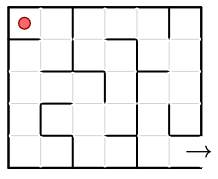
\includegraphics[width=0.25\textwidth]{../images/maze_empty.png}
        \captionof{figure}{Labyrinthe}
    \end{center}
    \textbf{Problème :} Peut-on sortir du labyrinthe ?\\
    \textbf{Solution :} On peut modéliser le labyrinthe par un graphe où chaque sommet représente une case du labyrinthe et chaque arête représente un passage entre deux cases adjacentes. Le labyrinthe est connexe si et seulement si il existe un chemin entre la case de départ et la case de sortie.
}

\definition{
    Une \textbf{composante connexe} d'un graphe est un sous-graphe connexe maximal (par inclusion).
}

\method{Réflexes pour étudier un problème de graphe}{
    \begin{enumerate}
        \item Trouver le graphe associé au problème.
        \item Identifier les sommets et les arêtes.
        \item \textit{dans la plupart des cas :} Vérifier si le graphe est connexe.
    \end{enumerate}
}

\definition{
    Soit $G = (V, E)$ un graphe. On considère l'application :
    $$\omega : E \longrightarrow \mathbb{R}$$
    qui associe à chaque arête un nombre réel. On appelle $\omega$ \textbf{la fonction de pondération} du graphe.
}
\vocabulary{Un graphe pondéré est un graphe muni d'une fonction de pondération.}

\definition{
    Un \textbf{graphe orienté} est un couple $(V, A)$ où $V$ est l'ensemble des sommets et $A \subset \{(u,v) \in V^2 \mid u \neq v\}$ est l'ensemble des arcs. Chaque arc est une paire ordonnée de sommets, indiquant une direction.
}
\remark{Sauf mention contraire, tous les graphes considérés dans ce cours sont simples (ni orientés, ni pondérés et sans boucles ni arêtes multiples).}

\subsection{Sous-graphes}

\definition{
    Soient $G = (V, E)$ et $H = (W, F)$ deux graphes. On dit que :
    \begin{itemize}
        \item $H$ est un \textbf{sous-graphe} de $G$ si $W \subseteq V$ et $F \subseteq \binom{W}{2} \cap E$, 
        \item $H$ est un \textbf{sous-graphe induit} (et on le note $G[W]$) de $G$ si $W \subseteq V$ et $F$ contient toutes les arêtes de $E$ dont les deux extrémités sont dans $W$ ($F = \binom{W}{2} \cap E$),
        \item $H$ est un \textbf{sous-graphe couvrant} de $G$ si $W = V$ et $F \subseteq E$.
    \end{itemize}
}

\remark{$\binom{W}{2} = \{ \{u, v\} \mid u, v \in W, u \neq v \}$ est l'ensemble de toutes les paires d'éléments distincts de $W$.\\ La différence avec $V^2$ est que $\binom{W}{2}$ ne contient pas les paires ordonnées et ne contient pas les paires avec des éléments identiques.}

\remark{
    De manière intuitive, un sous-graphe...
    \begin{itemize}
        \item est un graphe formé à partir d'un ensemble de sommets et d'arêtes du graphe original.
        \item induit est un sous-graphe qui contient toutes les arêtes entre les sommets choisis.
        \item couvrant est un sous-graphe qui contient tous les sommets du graphe original, mais seulement certaines arêtes.
    \end{itemize}
}

\theorem{Proposition}{Sous-graphe induit couvrant}{false}{
    Soit $G = (V, E)$. Le sous-graphe couvrant induit par $V$ est $G$ lui-même. En d'autres termes, $G[V] = G$.
}

\subsection{Graphes complets et complémentaires}

\definition{
    Un graphe $G = (V, E)$ est dit \textbf{complet} si pour tout couple de sommets distincts $(u, v) \in V^2$, il existe une arête entre $u$ et $v$. On note le graphe complet sur $n$ sommets par $K_n$.
}

\theorem{Proposition}{Caractérisation du graphe complet}{false}{
    Il vient : $$K_n = (\{1, 2, \ldots, n\}, \binom{\{1, 2, \ldots, n\}}{2})$$.
}

\theorem{Proposition}{Nombre d'arêtes dans un graphe complet}{false}{
    Le nombre d'arêtes dans un graphe complet à $n$ sommets est donné par la formule :
    $$|E(K_n)| = \binom{n}{2} = \frac{n(n-1)}{2} \in \Theta(n^2)$$
}

\definition{
    Soit $G = (V, E)$ un graphe. Le \textbf{graphe complémentaire} de $G$, noté $\overline{G}$, est le graphe défini par :
    $$\overline{G} = (V, \binom{V}{2} \setminus E)$$
}
\newpage
\section{Stockage des graphes}

\subsection{Vocabulaire et conventions}

\remark{Pour les noms de variables, on pose les conventions suivantes :
    \begin{itemize}
        \item $V$ \textit{(vertices)} : l'ensemble des sommets du graphe,
        \item $E$ \textit{(edges)}: l'ensemble des arêtes du graphe,
        \item $n = |V|$ : le nombre de sommets du graphe,
        \item $m = |E|$ : le nombre d'arêtes du graphe.
    \end{itemize}
}

\definition{
    Soient $G$ un graphe, $u$ et $v$ deux sommets de $G$ et $e$ une arête de $G$. On dit que :
    \begin{itemize}
        \item $u$ et $v$ sont \textbf{adjacents} (ou voisins) si $\{u, v\} \in E$,
        \item $e$ est \textbf{incident} à $u$ si $u \in e$,
        \item les deux éléments de $e$ sont ses \textbf{extrémités},
        \item le \textbf{voisinage} d'un sommet $u$ est l'ensemble des sommets adjacents à $u$, noté $N_G(u)$,
        \item les \textbf{voisins} de $u$ sont les éléments de $N_G(u)$.
    \end{itemize}
}

\subsection{Matrice d'adjacence}

\definition{
    Soit $G$ un graphe à $n$ sommets. On numérote les sommets $V(G) = \{v_0, v_1, \ldots, v_{n-1}\}$. La \textbf{matrice d'adjacence} de $G$, notée $A(G)$, est la matrice carrée $n \times n$ définie par :
    \[
    A(G)_{ij} = \begin{cases}
    1 & \text{si } \{v_i, v_j\} \in E(G) \\
    0 & \text{sinon}
    \end{cases}
    \]
}

\example{Pour le graphe $G$ suivant :
\begin{center}
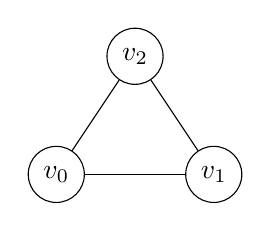
\begin{tikzpicture}
    \node[draw, circle] (v1) at (0, 0) {$v_0$};
    \node[draw, circle] (v2) at (2, 0) {$v_1$};
    \node[draw, circle] (v3) at (1, 1.5) {$v_2$};
    \draw (v1) -- (v2);
    \draw (v2) -- (v3);
    \draw (v3) -- (v1);
\end{tikzpicture}
\end{center}
La matrice d'adjacence est :
\[
A(G) = \begin{pmatrix}
0 & 1 & 1 \\
1 & 0 & 1 \\
1 & 1 & 0
\end{pmatrix}
\]
}
\remark{La matrice d'adjacence est symétrique pour un graphe non orienté, et sa diagonale est nulle.}

\subsection{Liste d'adjacence}

\definition{
    Soit $G$ un graphe à $n$ sommets. On numérote les sommets $V(G) = \{v_0, v_1, \ldots, v_{n-1}\}$.\\
    La \textbf{liste d'adjacence} de $G$ est une liste contenant, pour chaque sommet $v_i$, la liste de ses voisins.
}

\example{
    Pour le graphe $G$ précédent, la liste d'adjacence $L$ est :
    \[
    \begin{aligned}
        L[0] &= [1, 2] \\
        L[1] &= [0, 2] \\
        L[2] &= [0, 1]
    \end{aligned}
    \]
}

\subsection{Matrice d'incidence}

\definition{
    Soit $G$ un graphe à $n$ sommets et $m$ arêtes. On numérote les sommets $V(G) = \{v_0, v_1, \ldots, v_{n-1}\}$ et les arêtes $E(G) = \{e_0, e_1, \ldots, e_{m-1}\}$. La \textbf{matrice d'incidence} de $G$, notée $B(G)$, est la matrice $n \times m$ définie par :
    \[
    B(G)_{ij} = \begin{cases}
    1 & \text{si } v_i \in e_j \\
    0 & \text{sinon}
    \end{cases}
    \]
}

\remark{La somme des éléments de chaque colonne de la matrice d'incidence est toujours égale à 2 pour un graphe simple non orienté.}

\example{
    Pour le graphe $G$ précédent, la matrice d'incidence est :
    \[
    B(G) = \begin{pmatrix}
    1 & 0 & 1 \\
    1 & 1 & 0 \\
    0 & 1 & 1
    \end{pmatrix}
    \]
}

\subsection{Algorithme : calcul du degré d'un sommet}

\vocabulary{Le \textbf{degré} d'un sommet $v$, noté $\deg(v)$, est le nombre d'arêtes incidentes à $v$.}

\training{Pour chacune des trois représentations (matrice d'adjacence, liste d'adjacence, matrice d'incidence), proposer un algorithme pour calculer le degré moyen du graphe.}
\noindent\textbf{1. Matrice d'adjacence :}\\
\ndlr{cf. cours}
\noindent\textbf{2. Liste d'adjacence :}\\
\begin{lstlisting}[language=Python, caption=Calcul du degré moyen à partir de la liste d'adjacence (\textbf{naïf})]
def degre_moyen (L):
    if(len(L) == 0):
        return -1

	sum_degre = 0
	for i in range len(L):
		sum_degre += len(L[i])
	return sum_degre/len(L)
\end{lstlisting}
\noindent\textbf{3. Matrice d'incidence :}\\
\ndlr{cf. cours}

\theorem{Théorème}{Somme des degrés}{false}{
    Soit $G = (V, E)$ un graphe simple non orienté à $n$ sommets et $m$ arêtes. Alors :
    $$\sum_{v \in V} \deg(v) = 2m$$
}
\noindent{\textbf{Preuve :} Soit $S$ la somme de tous les éléments de la matrice d'incidence de $G$.\\
La somme de chaque ligne est égale au degré du sommet correspondant, donc $S = \sum_{v \in V} \deg(v)$.\\
La somme de chaque colonne est égale à 2, car chaque arête a exactement deux extrémités, donc $S = 2m$.\\
Ainsi, $\sum_{v \in V} \deg(v) = 2m$.}

\theorem{Corollaire}{Parité du degré}{false}{
    Soit $G = (V, E)$ un graphe. Alors :
    $$\sum_{v \in V} \deg(v) \in 2\mathbb{N}$$
    Autrement dit, le nombre de sommets de degré impair dans un graphe est pair.
}

\example{Sept personnes se serrent la main. Il n'est pas possible que chacun d'entre eux serre lla main exactement trois fois (et même un nombre impair de fois). En effet, si chacun serre la main trois fois, le nombre total de poignées de main serait $7 \times 3 = 21$, ce qui est impair. Or, d'après le corollaire précédent, le nombre total de poignées de main doit être pair.}

\subsection{Analyse de complexité}

\definition{
    La \textbf{complexité temporelle} (dans le pire ca) d'un algorithme $A$, noté $T(n)$, est le nombre d'opérations élémentaires maximum que puisse effectuer $A$ avant d'ariver à un résultat, étant donné une entrée de taille $N$.
}

\attention{Pour un graphe, on compte la complexité en fonction de $n$ et $m$ (respectivement le nombre de sommets et d'arêtes), et non pas en fonction de la taille de la représentation du graphe.}

\theorem{Proposition}{}{false}{
    Soit $G$ un graphe connexe. Alors :
    $$m \geq n - 1$$
}
\noindent{\textbf{Preuve :} Partons du graphe sans arête sur les mêmes $n$ sommets : il possède $n$ composantes connexes. Ajouter une arête réduit ce nombre d’au plus 1. Comme $G$ n’a qu’une seule composante, il faut donc au moins $n - 1$ arêtes.}

\section{Arbres}

\subsection{Définition et caractérisation}
\definition{Un \textbf{arbre} est un graphe connexe et acyclique.}

\vocabulary{Un sommet de degré 1 dans un arbre est appelé une \textbf{feuille}.}

\theorem{Théorème}{Caractérisation des arbres}{false}{
    Soit $G = (V, E)$ un graphe simple non orienté à $n$ sommets. Alors les propositions suivantes sont équivalentes :
    \begin{enumerate}
        \item $G$ est un arbre,
        \item Pour toute paire de sommets $u,v \in V(G)$, il existe un unique chemin reliant $u$ à $v$,
        \item $G$ est connexe, et toute suppression d'une arête de $G$ le rend non connexe,
        \item $G$ est acyclique, et tout ajout d'une arête à $G$ le rend cyclique,
        \item $G$ est acyclique et $|E(G)| = |V(G)| - 1$ ($m = n - 1$),
        \item $G$ est connexe et $m = n - 1$ ($n-1$ arêtes pour $n$ sommets).
    \end{enumerate}
}


\subsection{Algorithme : faire pousser un arbre}

\theorem{Lemme}{}{false}{Tout arbre avec au moins deux sommets contient au moins deux feuilles.}
\theorem{Lemme}{}{false}{\begin{center}$G$ est un arbre avec une feuille $v$ $\Leftrightarrow \; G - v$ est un arbre. \end{center}}

\subsection{Arbre couvrant}

\definition{Soit $G=(V, E)$ un graphe.Un \textbf{arbre couvrant} de $G$ est un sous-graphe couvrant de $G$ (ie. contenant tous les sommets de $G$) qui est un arbre.}
\example{
    \begin{figure}[htbp]
    \centering
    \tikzset{
        vertex/.style={circle, draw, fill=black, inner sep=0pt, minimum size=3pt},
        tree edge/.style={line width=1.5pt, red}
    }

    % 1. Graphe de départ G
    \begin{subfigure}[b]{0.45\textwidth}
        \centering
        \begin{tikzpicture}[scale=0.9]
            % Sommets
            \node[vertex, label=above:{$v_1$}] (v1) at (0,2) {};
            \node[vertex, label=above:{$v_2$}] (v2) at (2.5,2) {};
            \node[vertex, label=below:{$v_3$}] (v3) at (0,0) {};
            \node[vertex, label=below:{$v_4$}] (v4) at (2.5,0) {};
            \node[vertex, label=right:{$v_5$}] (v5) at (4,1) {};

            % Arêtes
            \draw (v1) -- (v2);
            \draw (v1) -- (v3);
            \draw (v2) -- (v3);
            \draw (v2) -- (v4);
            \draw (v3) -- (v4);
            \draw (v2) -- (v5);
            \draw (v4) -- (v5);
        \end{tikzpicture}
        \caption*{Graphe initial $G=(V,E)$}
    \end{subfigure}
    \hspace{0.2cm}
    % 2. Arbre couvrant T de G
    \begin{subfigure}[b]{0.45\textwidth}
        \centering
        \begin{tikzpicture}[scale=0.9]
            % Sommets (tous conservés)
            \node[vertex, label=above:{$v_1$}] (v1) at (0,2) {};
            \node[vertex, label=above:{$v_2$}] (v2) at (2.5,2) {};
            \node[vertex, label=below:{$v_3$}] (v3) at (0,0) {};
            \node[vertex, label=below:{$v_4$}] (v4) at (2.5,0) {};
            \node[vertex, label=right:{$v_5$}] (v5) at (4,1) {};

            % Arêtes non retenues (pointillées/grises)
            \draw[gray!40, dashed] (v2) -- (v3);
            \draw[gray!40, dashed] (v3) -- (v4);
            \draw[gray!40, dashed] (v4) -- (v5);

            % Arêtes de l'arbre couvrant (rouges et épaissies)
            \draw[tree edge] (v1) -- (v2);
            \draw[tree edge] (v1) -- (v3);
            \draw[tree edge] (v2) -- (v4);
            \draw[tree edge] (v2) -- (v5);
        \end{tikzpicture}
        \caption*{Un arbre couvrant $T=(V, E')$}
    \end{subfigure}
    \end{figure}
}

\theorem{Proposition}{Lien entre connexité et arbre couvrant}{false}{
    Un graphe $G$ est connexe si et seulement s'il possède un arbre couvrant.
}
\noindent{\textbf{Preuve :} Soit $G$ un graphe connexe.
\begin{itemize}
    \item Retirons de $G$, tant que possible, une arête qui ne rend pas le graphe non connexe.
    \item On obtient $T$ un sous-graphe connexe de $G$ qui est acyclique (sinon on pourrait retirer une arête du cycle sans rendre le graphe non connexe).
    \item Donc $T$ est un arbre couvrant de $G$.
    \item La réciproque est immédiate : si $G$ possède un arbre couvrant, alors $G$ est connexe.
\end{itemize}}

\section{Algorithme : décider si un graphe est connexe}
\subsection{Marquage des sommets}

cf. page 80 (17) du cours 2

\subsection{Algorithme BFS : parcours en largeur}

cf. page 83 (20) du cours 2

\newpage
\tableofcontents
\section*{Crédits}
Ce cours est inspiré des slides de cours de l'Université Paris Cité réalisés par Mónika Csikós et Mikäel Rabie. Assurez-vous de citer correctement la source si vous utilisez ce cours dans vos travaux.\\\\
Ce cours est mis à disposition selon les termes de la Licence Creative Commons \ccbyncsa\ \textbf{Attribution - Pas d'Utilisation Commerciale - Partage dans les Mêmes Conditions 4.0 International}. 
Pour voir une copie de cette licence, visitez \url{http://creativecommons.org/licenses/by-nc-sa/4.0/}.

\end{document}